% !TeX encoding = UTF-8
% !TeX program = xelatex
% !TeX spellcheck = en_US

\documentclass[degree=master,language=english,cjk-font=external]{sustechthesis}
  % 学位 degree:
  %   master (默认) | doctor
  % 语言 language:
  %   chinese (默认)| english
  % 中文字体 cjk-font
  %   auto (默认,自动选择系统自带字体)| external (包内字体)| windows | mac | 等
  %   在 **非Windows** 的系统上推荐使用包内字体,而非系统字体。
  %   以达到和 Windows 系统上显示的字体效果。
  %   Windows 系统上可以删除该参数,使用系统内置字体。


% 论文基本配置,加载宏包等全局配置
% !TeX root = ./sustechthesis-example.tex

% 论文基本信息配置

\thusetup{
  %******************************
  % 注意:
  %   1. 配置里面不要出现**空行**
  %   2. 不需要的配置信息可以删除
  %   3. 建议先阅读文档中所有关于选项的说明
  %******************************
  %
  % 输出格式
  %   选择打印版(print)或用于提交的电子版(electronic),前者会插入空白页以便直接双面打印
  %
  output = electronic,
  %
  % 标题
  %   可使用“\\”命令手动控制换行
  %   如果需要使用副标题,取消 subtitle 和 subtitle* 的注释即可。
  %
  title  = {南方科技大学学位论文 \LaTeX{} 模板 (Support English) 使用示例文档 v\version},
  title* = {An Introduction to \LaTeX{} Thesis Template of Southern University of Science and Technology v\version},
  % subtitle = {可选的副标题可选的副标题可选的副标题可选的副标题可选的副标题可选的副标题},
  % subtitle* = {optional subtitle optional subtitle optional subtitle optional subtitle optional subtitle optional subtitle},
  %
  % 学位
  %
  degree-domain = {工学}, % 【中文】学科门类:可选理学、工学、医学
  degree-domain* = {Engineering}, % 【英文】学位等级:可选Science, Engineering, Medicine
  gongshuo = false, % 是否为专业型学位。专业型学位则填 true ,学术型或其他为 false 。
  %
  % 培养单位
  %   填写所属院系的全名
  %   超长英文系名可以手动换行
  department = {计算机科学与工程系},
  department* = {School of System Design and \\Intelligent Manufacturing},
  %
  % 学科
  %   1. 学术型学位
  %      获得一级学科授权的学科填写一级学科名称,其他填写二级学科名称
  %   2. 工程硕士
  %      工程领域名称
  %
  discipline  = {计算机科学与技术},
  discipline* = {Computer Science and Technology},
  %
  % 姓名
  %   英文用全拼,姓在前,名在后,姓和名的首字母大写,其余小写
  %
  author  = {李子强},
  author* = {Li Ziqiang},
  %
  % 指导教师
  %   一般情况下,只写一名指导教师。
  %   填写导师姓名,后衬导师职称“教授”,“副教授”,“研究员”等
  %
  supervisor  = {爱丽丝鲍勃助理教授},
  supervisor* = {Assistant Prof. Alice Bob},
  % 副指导教师
  %   限一名,且需要向学位办确认和备案,职称要求同指导教师。
  associate-supervisor  = {大卫查理助理教授},
  associate-supervisor* = {Assistant Prof. David Charlie},
  %
  % 日期
  %   使用 ISO 格式;默认为当前时间
  %   date 为第一页全中文大写日期,defense-date 为第二、三页的答辩日期。
  %   需要按 {年-月-日} 格式填写,如不显示“日”,可以随意填一个日期,但是不能为空。
  %
  date = {2020-12-20},
  defense-date = {2020-12-20},
  %
  % 密级
  %   公开, 秘密, 机密, 绝密
  %
  statesecrets={公开},
  %
  % 国内图书分类号,国际图书分类号
  %
  natclassifiedindex={TM301.2},
  intclassifiedindex={62-5},
}

% 载入所需的宏包

% 可以使用 nomencl 生成符号和缩略语说明
% \usepackage{nomencl}
% \makenomenclature

% 表格加脚注
\usepackage{threeparttable}

% 表格中支持跨行
\usepackage{multirow}

% 量和单位
\usepackage{siunitx}

% 定理类环境宏包
\usepackage{amsthm}
% 也可以使用 ntheorem
% \usepackage[amsmath,thmmarks,hyperref]{ntheorem}

%%%%%% 参考文献编译方式二选一,不要同时开启。
%%%% 选择一
%% 参考文献使用 BibTeX + natbib 宏包
%% 顺序编码制
\usepackage[sort&compress]{gbt7714}
\citestyle{super}
\bibliographystyle{sustechthesis-numeric}
\usepackage{bibunits}
\defaultbibliographystyle{sustechthesis-numeric}

%%%% 选择二(不兼容本模板,请勿使用)
%% 参考文献使用 BibLaTeX 宏包
% \usepackage[backend=biber,style=gb7714-2015]{biblatex}
%% 声明 BibLaTeX 的数据库
% \addbibresource{ref/refs.bib}

% 定义所有的图片文件在 figures 子目录下
\graphicspath{{figures/}}

% 数学命令
\newcommand\dif{\mathop{}\!\mathrm{d}}  % 微分符号

% hyperref 宏包在最后调用
\usepackage{hyperref}
\usepackage{ragged2e}

% 固定宽度的表格。放在 hyperref 之前的话,tabularx 里的 footnote 显示不出来。
\usepackage{tabularx}

% 跨页表格,必须在 hyperref 之后使用否则会报错。
\usepackage{longtable}

% 源代码高亮
\usepackage{minted}

% 伪代码环境
\usepackage[ruled,linesnumbered]{algorithm2e}



\begin{document}

% 封面
\maketitle

% 学位论文公开评阅人和答辩委员会名单
% !TeX root = ../sustechthesis-example.tex

% 填写说明:
% 1、各类名单按实际人数逐行填写,可增加或删除行,不留空行。
% 2、“公开评阅人名单”仅填写公开评阅人信息,不填写隐名评阅人信息。
% 3、填写完毕后请及时删除提示红框。

\begin{committee}[name={学位论文公开评阅人和答辩委员会名单}]

  \vspace{18bp}

  \newcolumntype{C}[1]{@{}>{\centering\arraybackslash}p{#1}}

  \section*{公开评阅人名单}

  \begin{center}
    \begin{tabular}{C{3cm}C{3cm}C{9cm}@{}}
      刘XX & 教授   & 南方科技大学                    \\
      陈XX & 副教授 & XXXX大学                    \\
      杨XX & 研究员 & 中国XXXX科学院XXXXXXX研究所 \\
    \end{tabular}
  \end{center}


  \section*{答辩委员会名单}

  \begin{center}
    \begin{tabular}{C{2.75cm}C{2.98cm}C{4.63cm}C{4.63cm}@{}}
      主席 & 赵XX                  & 教授                    & 南方科技大学       \\
      委员 & 刘XX                  & 教授                    & 南方科技大学       \\
          & \multirow{2}{*}{杨XX} & \multirow{2}{*}{研究员} & 中国XXXX科学院 \\
          &                       &                         & XXXXXXX研究所  \\
          & 黄XX                  & 教授                    & XXXX大学       \\
          & 周XX                  & 副教授                  & XXXX大学       \\
      秘书 & 吴XX                  & 助理研究员              & 南方科技大学       \\
    \end{tabular}
  \end{center}

\end{committee}



% 也可以导入 Word 版转的 PDF 文件
% \begin{committee}[file=figures/scan-committee.pdf]
% \end{committee}


% 南方科技大学学位论文原创性声明和使用授权说明
% 本模版不会对扫描版的页码进行处理,建议定稿后打印声明页再插入编译,以免页码出错。
% 或者,使用其他 pdf 拼接软件也可达到替换声明页面的目的。
\statementcopyright % 生成未签名的声明
% \statementcopyright[scan-statement.pdf] % 插入已签名的声明文件(扫描版)

\frontmatter
% !TeX root = ../sustechthesis-example.tex

% 中英文摘要和关键字

\begin{abstract}
  论文的摘要是对论文研究内容和成果的高度概括。
  摘要应对论文所研究的问题及其研究目的进行描述,对研究方法和过程进行简单介绍,对研究成果和所得结论进行概括。
  摘要应具有独立性和自明性,其内容应包含与论文全文同等量的主要信息。
  使读者即使不阅读全文,通过摘要就能了解论文的总体内容和主要成果。

  论文摘要的书写应力求精确、简明。
  切忌写成对论文书写内容进行提要的形式,尤其要避免“第 1 章……;第 2 章……;……”这种或类似的陈述方式。

  关键词是为了文献标引工作、用以表示全文主要内容信息的单词或术语。
  关键词不超过 5 个,每个关键词中间用分号分隔。

  % 关键词用“英文逗号”分隔,输出时会自动处理为正确的分隔符
  \thusetup{
    keywords = {关键词 1, 关键词 2, 关键词 3, 关键词 4, 关键词 5},
  }
\end{abstract}

\begin{abstract*}
  An abstract of a dissertation is a summary and extraction of research work and contributions.
  Included in an abstract should be description of research topic and research objective, brief introduction to methodology and research process, and summarization of conclusion and contributions of the research.
  An abstract should be characterized by independence and clarity and carry identical information with the dissertation.
  It should be such that the general idea and major contributions of the dissertation are conveyed without reading the dissertation.

  An abstract should be concise and to the point.
  It is a misunderstanding to make an abstract an outline of the dissertation and words “the first chapter”, “the second chapter” and the like should be avoided in the abstract.

  Keywords are terms used in a dissertation for indexing, reflecting core information of the dissertation.
  An abstract may contain a maximum of 5 keywords, with semi-colons used in between to separate one another.

  % Use comma as seperator when inputting
  \thusetup{
    keywords* = {keyword 1, keyword 2, keyword 3, keyword 4, keyword 5},
  }
\end{abstract*}


% 目录
\tableofcontents

% 插图和附表清单
% \listoffiguresandtables  % 插图和附表清单
% \listoffigures           % 插图清单
% \listoftables            % 附表清单

% 符号对照表
% % !TeX root = ../sustechthesis-example.tex

% denotation 环境带一个可选参数,用来指定符号列的宽度(默认为 2.5cm),下面改3cm为例。
% 如果论文中使用了大量的物理量符号、标志、缩略词、专门计量单位、自定义名词和术语等, 应编写“符号和缩略语说明”。
% 论文中主要符号应全部采用法定单位, 严格执行《量和单位》(GB3100~3102-93)的有关规定、单位名称的书写,可以采用国际通用符号,也可以用中文名称,但全文应统一,不得两种混用。
% 缩略语应列出中英文全称。符号和缩略语说明排序方法先按拉丁字母大写、小写排序, 再按希腊字母大写、小写排序, 如下表所示:
% ABCDEFGHIJKLMNOPQRSRUVWXYZ
% abcdefghijklmnopqrstuvwxyz
% Alpha
% Beta
% Gamma
% Delta
% Epsilon
% Zeta
% Eta
% Theta
% Iota
% Kappa
% Lambda
% Mu
% Nu
% Xi
% Omicron
% Pi
% Rho
% Sigma
% Tau
% Upsilon
% Phi
% Chi
% Psi
% Omega
% alpha
% beta
% gamma
% delta
% epsilon
% zeta
% eta
% theta
% iota
% kappa
% lambda
% mu
% nu
% xi
% omicron
% pi
% rho
% sigma
% tau
% upsilon
% phi
% chi
% psi
% omega

% 希腊字母详见 https://xilazimu.net/


\begin{denotation}[3cm]
  \item[As-PPT]聚苯基不对称三嗪
  \item[DFT]密度泛函理论 (Density Functional Theory)
  \item[DMAsPPT]聚苯基不对称三嗪双模型化合物(水解实验模型化合物)
  \item[$E_a$]化学反应的活化能 (Activation Energy)
  \item[HMAsPPT]聚苯基不对称三嗪模型化合物的质子化产物
  \item[HMPBI]聚苯并咪唑模型化合物的质子化产物
  \item[HMPI]聚酰亚胺模型化合物的质子化产物
  \item[HMPPQ]聚苯基喹噁啉模型化合物的质子化产物
  \item[HMPY]聚吡咙模型化合物的质子化产物
  \item[HMSPPT]聚苯基对称三嗪模型化合物的质子化产物
  \item[HPCE]高效毛细管电泳色谱 (High Performance Capillary lectrophoresis)
  \item[HPLC]高效液相色谱 (High Performance Liquid Chromatography)
  \item[IRC]内禀反应坐标 (Intrinsic Reaction Coordinates)
  \item[LC-MS]液相色谱-质谱联用 (Liquid chromatography-Mass Spectrum)
  \item[MAsPPT]聚苯基不对称三嗪单模型化合物,3,5,6-三苯基-1,2,4-三嗪
  \item[MPBI]聚苯并咪唑模型化合物,N-苯基苯并咪唑
  \item[MPI]聚酰亚胺模型化合物,N-苯基邻苯酰亚胺
  \item[MPPQ]聚苯基喹噁啉模型化合物,3,4-二苯基苯并二嗪
  \item[MPY]聚吡咙模型化合物
  \item[MSPPT]聚苯基对称三嗪模型化合物,2,4,6-三苯基-1,3,5-三嗪
  \item[ONIOM]分层算法 (Our own N-layered Integrated molecular Orbital and molecular Mechanics)
  \item[PBI]聚苯并咪唑
  \item[PDT]热分解温度
  \item[PES]势能面 (Potential Energy Surface)
  \item[PI]聚酰亚胺
  \item[PMDA-BDA]均苯四酸二酐与联苯四胺合成的聚吡咙薄膜
  \item[PPQ]聚苯基喹噁啉
  \item[PY]聚吡咙
  \item[S-PPT]聚苯基对称三嗪
  \item[SCF]自洽场 (Self-Consistent Field)
  \item[SCRF]自洽反应场 (Self-Consistent Reaction Field)
  \item[TIC]总离子浓度 (Total Ion Content)
  \item[TS]过渡态 (Transition State)
  \item[TST]过渡态理论 (Transition State Theory)
  \item[ZPE]零点振动能 (Zero Vibration Energy)
  \item[\textit[ab initio]]基于第一原理的量子化学计算方法,常称从头算法
  \item[$\Delta G^\neq$]活化自由能(Activation Free Energy)
  \item[$\kappa$]传输系数 (Transmission Coefficient)
  \item[$\nu_i$]虚频 (Imaginary Frequency)
\end{denotation}



% 也可以使用 nomencl 宏包,需要在导言区
% \usepackage{nomencl}
% \makenomenclature

% 在这里输出符号说明
% \printnomenclature[3cm]

% 在正文中的任意为都可以标题
% \nomenclature{As-PPT}{聚苯基不对称三嗪}
% \nomenclature{DFT}{密度泛函理论 (Density Functional Theory)}
% \nomenclature{DMAsPPT}{聚苯基不对称三嗪双模型化合物(水解实验模型化合物)}
% \nomenclature{$E_a$}{化学反应的活化能 (Activation Energy)}
% \nomenclature{HMAsPPT}{聚苯基不对称三嗪模型化合物的质子化产物}
% \nomenclature{HMPBI}{聚苯并咪唑模型化合物的质子化产物}
% \nomenclature{HMPI}{聚酰亚胺模型化合物的质子化产物}
% \nomenclature{HMPPQ}{聚苯基喹噁啉模型化合物的质子化产物}
% \nomenclature{HMPY}{聚吡咙模型化合物的质子化产物}
% \nomenclature{HMSPPT}{聚苯基对称三嗪模型化合物的质子化产物}
% \nomenclature{HPCE}{高效毛细管电泳色谱 (High Performance Capillary lectrophoresis)}
% \nomenclature{HPLC}{高效液相色谱 (High Performance Liquid Chromatography)}
% \nomenclature{IRC}{内禀反应坐标 (Intrinsic Reaction Coordinates)}
% \nomenclature{LC-MS}{液相色谱-质谱联用 (Liquid chromatography-Mass Spectrum)}
% \nomenclature{MAsPPT}{聚苯基不对称三嗪单模型化合物,3,5,6-三苯基-1,2,4-三嗪}
% \nomenclature{MPBI}{聚苯并咪唑模型化合物,N-苯基苯并咪唑}
% \nomenclature{MPI}{聚酰亚胺模型化合物,N-苯基邻苯酰亚胺}
% \nomenclature{MPPQ}{聚苯基喹噁啉模型化合物,3,4-二苯基苯并二嗪}
% \nomenclature{MPY}{聚吡咙模型化合物}
% \nomenclature{MSPPT}{聚苯基对称三嗪模型化合物,2,4,6-三苯基-1,3,5-三嗪}
% \nomenclature{ONIOM}{分层算法 (Our own N-layered Integrated molecular Orbital and molecular Mechanics)}
% \nomenclature{PBI}{聚苯并咪唑}
% \nomenclature{PDT}{热分解温度}
% \nomenclature{PES}{势能面 (Potential Energy Surface)}
% \nomenclature{PI}{聚酰亚胺}
% \nomenclature{PMDA-BDA}{均苯四酸二酐与联苯四胺合成的聚吡咙薄膜}
% \nomenclature{PPQ}{聚苯基喹噁啉}
% \nomenclature{PY}{聚吡咙}
% \nomenclature{S-PPT}{聚苯基对称三嗪}
% \nomenclature{SCF}{自洽场 (Self-Consistent Field)}
% \nomenclature{SCRF}{自洽反应场 (Self-Consistent Reaction Field)}
% \nomenclature{TIC}{总离子浓度 (Total Ion Content)}
% \nomenclature{TS}{过渡态 (Transition State)}
% \nomenclature{TST}{过渡态理论 (Transition State Theory)}
% \nomenclature{ZPE}{零点振动能 (Zero Vibration Energy)}
% \nomenclature{\textit{ab initio}}{基于第一原理的量子化学计算方法,常称从头算法}
% \nomenclature{$\Delta G^\neq$}{活化自由能(Activation Free Energy)}
% \nomenclature{$\kappa$}{传输系数 (Transmission Coefficient)}
% \nomenclature{$\nu_i$}{虚频 (Imaginary Frequency)}



% 正文部分
\mainmatter
% !TeX root = ../sustechthesis-example.tex

\chapter{论文主要部分的写法}

研究生学位论文撰写,除表达形式上需要符合一定的格式要求外,内容方面上也要遵循一些共性原则。

通常研究生学位论文只能有一个主题(不能是几块工作拼凑在一起),该主题应针对某学科领域中的一个具体问题展开深入、系统的研究,并得出有价值的研究结论。
学位论文的研究主题切忌过大,例如,“中国国有企业改制问题研究”这样的研究主题过大,因为“国企改制”涉及的问题范围太广,很难在一本研究生学位论文中完全研究透彻。



\section{论文的语言及表述}

除国际研究生外,学位论文一律须用汉语书写。
学位论文应当用规范汉字进行撰写,除古汉语研究中涉及的古文字和参考文献中引用的外文文献之外,均采用简体汉字撰写。

国际研究生一般应以中文或英文书写学位论文,格式要求同上。
论文须用中文封面。

研究生学位论文是学术作品,因此其表述要严谨简明,重点突出,专业常识应简写或不写,做到立论正确、数据可靠、说明透彻、推理严谨、文字凝练、层次分明,避免使用文学性质的或带感情色彩的非学术性语言。

论文中如出现一个非通用性的新名词、新术语或新概念,需随即解释清楚。



\section{论文题目的写法}

论文题目应简明扼要地反映论文工作的主要内容,力求精炼、准确,切忌笼统。
论文题目是对研究对象的准确、具体描述,一般要在一定程度上体现研究结论,因此,论文题目不仅应告诉读者这本论文研究了什么问题,更要告诉读者这个研究得出的结论。
例如:“在事实与虚构之间:梅乐、卡彭特、沃尔夫的新闻观”就比“三个美国作家的新闻观研究”更专业、更准确。



\section{摘要的写法}

论文摘要是对论文研究内容的高度概括,应具有独立性和自含性,即应是 一篇简短但意义完整的文章。
通过阅读论文摘要,读者应该能够对论文的研究 方法及结论有一个整体性的了解,因此摘要的写法应力求精确简明。
论文摘要 应包括对问题及研究目的的描述、对使用的方法和研究过程进行的简要介绍、 对研究结论的高度凝练等,重点是结果和结论。

论文摘要切忌写成全文的提纲,尤其要避免“第 1 章……;第 2 章……;……”这样的陈述方式。



\section{引言的写法}

一篇学位论文的引言大致包含如下几个部分:
1、问题的提出;
2、选题背 景及意义;
3、文献综述;
4、研究方法;
5、论文结构安排。
\begin{itemize}
  \item 问题的提出:要清晰地阐述所要研究的问题“是什么”。
    % \footnote{选题时切记要有“问题意识”,不要选不是问题的问题来研究。}
  \item 选题背景及意义:论述清楚为什么选择这个题目来研究,即阐述该研究对学科发展的贡献、对国计民生的理论与现实意义等。
  \item 文献综述:对本研究主题范围内的文献进行详尽的综合述评,“述”的同时一定要有“评”,指出现有研究状态,仍存在哪些尚待解决的问题,讲出自己的研究有哪些探索性内容。
  \item 研究方法:讲清论文所使用的学术研究方法。
  \item 论文结构安排:介绍本论文的写作结构安排。
\end{itemize}



\section{正文的写法}

本部分是论文作者的研究内容,不能将他人研究成果不加区分地掺和进来。
已经在引言的文献综述部分讲过的内容,这里不需要再重复。
各章之间要存在有机联系,符合逻辑顺序。



\section{结论的写法}

结论是对论文主要研究结果、论点的提炼与概括,应精炼、准确、完整,使读者看后能全面了解论文的意义、目的和工作内容。
结论是最终的、总体的结论,不是正文各章小结的简单重复。
结论应包括论文的核心观点,主要阐述作者的创造性工作及所取得的研究成果在本领域中的地位、作用和意义,交代研究工作的局限,提出未来工作的意见或建议。
同时,要严格区分自己取得的成果与指导教师及他人的学术成果。

在评价自己的研究工作成果时,要实事求是,除非有足够的证据表明自己的研究是“首次”、“领先”、“填补空白”的,否则应避免使用这些或类似词语。

% !TeX root = ../sustechthesis-example.tex

\chapter{图表示例}

\section{插图}

图片通常在 \env{figure} 环境中使用 \cs{includegraphics} 插入,如图~\ref{fig:example} 的源代码。
建议矢量图片使用 PDF 格式,比如数据可视化的绘图;
照片应使用 JPG 格式;
其他的栅格图应使用无损的 PNG 格式。
注意,LaTeX 不支持 TIFF 格式;EPS 格式已经过时。

\begin{figure}
  \centering
  
\includegraphics[width=0.6\linewidth]{example-image-a.pdf}
  \caption{示例图片}
  \label{fig:example}
\end{figure}

若图或表中有附注,采用英文小写字母顺序编号,附注写在图或表的下方。
% LaTeX 传统上一般将附注的内容同图表的标题写在一起,形成很长的一段文字。

如果一个图由两个或两个以上分图组成时,各分图分别以(a)、(b)、(c)...... 作为图序,并须有分图题。
推荐使用 \pkg{subcaption} 宏包来处理, 比如图~\ref{fig:subfig-a} 和图~\ref{fig:subfig-b}。

\begin{figure}
  \centering
  \subcaptionbox{分图 A\label{fig:subfig-a}}
    {
\includegraphics[width=0.45\linewidth]{example-image-a.pdf}}
  \subcaptionbox{分图 B\label{fig:subfig-b}}
    {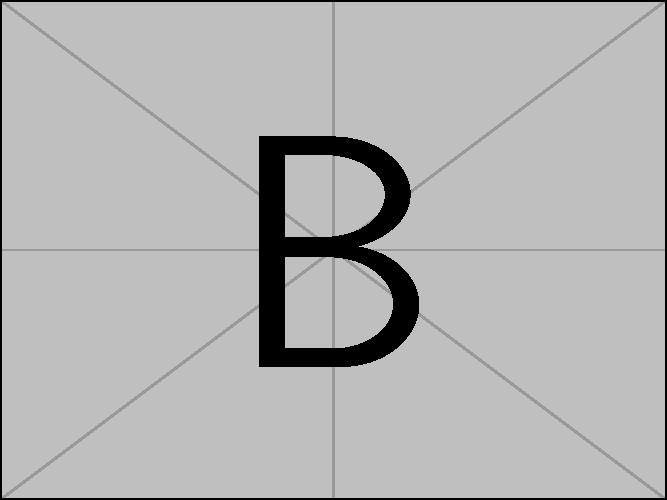
\includegraphics[width=0.45\linewidth]{example-image-b.pdf}}
  \caption{多个分图的示例}
  \label{fig:multi-image}
\end{figure}



\section{表格}

表应具有自明性。为使表格简洁易读,尽可能采用三线表,如表~\ref{tab:three-line}。
三条线可以使用 \pkg{booktabs} 宏包提供的命令生成。

\begin{table}
  \centering
  \caption{三线表示例}
  \begin{tabular}{ll}
    \toprule
    文件名          & 描述                         \\
    \midrule
    thuthesis.dtx   & 模板的源文件,包括文档和注释 \\
    thuthesis.cls   & 模板文件                     \\
    thuthesis-*.bst & BibTeX 参考文献表样式文件    \\
    thuthesis-*.bbx & BibLaTeX 参考文献表样式文件  \\
    thuthesis-*.cbx & BibLaTeX 引用样式文件        \\
    \bottomrule
  \end{tabular}
  \label{tab:three-line}
\end{table}

表格如果有附注,尤其是需要在表格中进行标注时,可以使用 \pkg{threeparttable} 宏包。使用英文小写字母 a、b、c……顺序编号。

\begin{table}
  \centering
  \begin{threeparttable}[c]
    \caption{带附注以及调整列宽的的表格示例}
    \label{tab:three-part-table}
  \begin{tabular}{C{2cm} L{4cm} R{6cm}}
    \toprule
    2cm          & 4cm & 6cm                         \\
    \midrule
    左右居中的2cm宽度左右居中的2cm宽度\tnote{a}   & 左右居左的4cm宽度左右居左的4cm宽度 & 左右居右的6cm宽度左右居右的6cm宽度\\
    左右居中的2cm宽度左右居中的2cm宽度\tnote{b}   & 左右居左的4cm宽度左右居左的4cm宽度 & 左右居右的6cm宽度左右居右的6cm宽度\\
    \bottomrule
  \end{tabular}
    \begin{tablenotes}
      \item [a] A的注释
      \item [b] B的注释
    \end{tablenotes}
  \end{threeparttable}
\end{table}
如果需要调整表格列宽度, 可以改用命令 \verb|L|, \verb|R|, 或者 \verb|C|, 如 \verb|C{2cm}| 代表居中列宽2cm。

\begin{table}
  \centering
  \caption{合并单元格的三线表}
  \label{tab:merge-cell}
  \begin{tabular}{lcccc}
  \toprule
    Metaclass & \multicolumn{2}{c}{A-B} & \multicolumn{2}{c}{C-D} \\ \cmidrule(l){1-1} \cmidrule(lr){2-3} \cmidrule(r){4-5}
    Class & A & B & C & D \\ \midrule
    L1 & 1 & 2 & 3 & 4 \\
    L2 & 1 & 2 & 3 & 4 \\
  \bottomrule
  \end{tabular}
\end{table}

如有辅助线要求可以使用 \verb|\cmidrule| 命令。在连续使用时,可以使用一组圆括号括起来的参数 \verb|l|、\verb|r|或\verb|l<距离>|、\verb|r<距离>|表示间距的表格线可以在左右向内缩短一小段,表\ref{tab:merge-cell}展示了效果。

表格如果想要与页面等宽,可以使用 \pkg{tabularx} 宏包,如表格\ref{tab:textwith-example}所示。
模版定义了一些扩展命令,实现一些排版需求。\verb|X| 两端对齐, \verb|Y| 左对齐, \verb|Z| 右对齐,或者 \verb|W| 居中对齐。

\begin{table}
  \centering
  \caption{同页宽的表格实例}
  \label{tab:textwith-example}
  \begin{tabularx}{\textwidth}{YXZW}
    \toprule
    Cell with text aligned to the left & 1 & 2 & 3\\ \midrule
    4 & Cell with justified text & 5 & 6\\ \midrule
    7 & 8 & Cell with centered text & 9\\ \midrule
    10 & 11 & 12 & Cell with text aligned to the right \\
    \bottomrule
  \end{tabularx}
\end{table}

如果您要排版的表格长度超过一页,那么推荐使用 \pkg{longtable} 或者 \pkg{supertabular}
宏包,模板对 \pkg{longtable} 进行了相应的设置,所以用起来可能简单一些。
表~\ref{tab:performance} 就是 \pkg{longtable} 的简单示例。

\begin{longtable}[c]{ccccclr}
  \caption{实验数据(超长表格示例)}\label{tab:performance}\\
  \toprule[1.5pt]
   测试程序 & \multicolumn{1}{c}{正常运行} & \multicolumn{1}{c}{同步} & \multicolumn{1}{c}{检查点} & \multicolumn{1}{c}{卷回恢复}
  & \multicolumn{1}{c}{进程迁移} & \multicolumn{1}{c}{检查点} \\
  & \multicolumn{1}{c}{时间 (s)}& \multicolumn{1}{c}{时间 (s)}&
  \multicolumn{1}{c}{时间 (s)}& \multicolumn{1}{c}{时间 (s)}& \multicolumn{1}{c}{
    时间 (s)}&  文件(KB)\\\midrule[1pt]
  \endfirsthead
  \multicolumn{7}{c}{续表~\thetable\hskip1em 实验数据(超长表格示例)}\\
  \toprule[1.5pt]
   测试程序 & \multicolumn{1}{c}{正常运行} & \multicolumn{1}{c}{同步} & \multicolumn{1}{c}{检查点} & \multicolumn{1}{c}{卷回恢复}
  & \multicolumn{1}{c}{进程迁移} & \multicolumn{1}{c}{检查点} \\
  & \multicolumn{1}{c}{时间 (s)}& \multicolumn{1}{c}{时间 (s)}&
  \multicolumn{1}{c}{时间 (s)}& \multicolumn{1}{c}{时间 (s)}& \multicolumn{1}{c}{
    时间 (s)}&  文件(KB)\\\midrule[1pt]
  \endhead
  \bottomrule[1.5pt]
  \multicolumn{7}{r}{续下页}
  \endfoot
  \endlastfoot
  CG.A.2 & 23.05 & 0.002 & 0.116 & 0.035 & 0.589 & 32491 \\
  CG.A.4 & 15.06 & 0.003 & 0.067 & 0.021 & 0.351 & 18211 \\
  CG.A.8 & 13.38 & 0.004 & 0.072 & 0.023 & 0.210 & 9890 \\
  CG.B.2 & 867.45 & 0.002 & 0.864 & 0.232 & 3.256 & 228562 \\
  CG.B.4 & 501.61 & 0.003 & 0.438 & 0.136 & 2.075 & 123862 \\
  CG.B.8 & 384.65 & 0.004 & 0.457 & 0.108 & 1.235 & 63777 \\
  MG.A.2 & 112.27 & 0.002 & 0.846 & 0.237 & 3.930 & 236473 \\
  MG.A.4 & 59.84 & 0.003 & 0.442 & 0.128 & 2.070 & 123875 \\
  MG.A.8 & 31.38 & 0.003 & 0.476 & 0.114 & 1.041 & 60627 \\
  MG.B.2 & 526.28 & 0.002 & 0.821 & 0.238 & 4.176 & 236635 \\
  MG.B.4 & 280.11 & 0.003 & 0.432 & 0.130 & 1.706 & 123793 \\
  MG.B.8 & 148.29 & 0.003 & 0.442 & 0.116 & 0.893 & 60600 \\
  LU.A.2 & 2116.54 & 0.002 & 0.110 & 0.030 & 0.532 & 28754 \\
  LU.A.4 & 1102.50 & 0.002 & 0.069 & 0.017 & 0.255 & 14915 \\
  LU.A.8 & 574.47 & 0.003 & 0.067 & 0.016 & 0.192 & 8655 \\
  LU.B.2 & 9712.87 & 0.002 & 0.357 & 0.104 & 1.734 & 101975 \\
  LU.B.4 & 4757.80 & 0.003 & 0.190 & 0.056 & 0.808 & 53522 \\
  LU.B.8 & 2444.05 & 0.004 & 0.222 & 0.057 & 0.548 & 30134 \\
  EP.A.2 & 123.81 & 0.002 & 0.010 & 0.003 & 0.074 & 1834 \\
  EP.A.4 & 61.92 & 0.003 & 0.011 & 0.004 & 0.073 & 1743 \\
  EP.A.8 & 31.06 & 0.004 & 0.017 & 0.005 & 0.073 & 1661 \\
  EP.B.2 & 495.49 & 0.001 & 0.009 & 0.003 & 0.196 & 2011 \\
  EP.B.4 & 247.69 & 0.002 & 0.012 & 0.004 & 0.122 & 1663 \\
  EP.B.8 & 126.74 & 0.003 & 0.017 & 0.005 & 0.083 & 1656 \\
  EP.A.2 & 123.81 & 0.002 & 0.010 & 0.003 & 0.074 & 1834 \\
  \bottomrule[1.5pt]
\end{longtable}


\section{源代码}

推荐使用 \pkg{listing} 环境嵌入 \pkg{minted} 环境高亮代码。\verb|linenos| 参数控制代码行号显示。\pkg{minted} 环境需要 Python 环境编译,并安装 Pygement 包,否则会编译失败。
引用效果如代码 \ref{lst:sample-code-minted}。

也可以使用 \pkg{listings} 环境高亮代码。参数较为复杂,请自行搜索或查阅文档。引用效果如代码 \ref{lst:sample-code-listings}。示例使用 \pkg{minipage} 环境嵌套一层的原因是防止换页中被插入其他浮动体,实际情况按需使用。但是,\textbf{不建议}混用 \pkg{listings} 环境和 \pkg{minted} 环境,会导致如上编号重复的错误,二选一即可。

\begin{listing}[!ht]
\caption{C++ 代码示例(使用 \pkg{minted} 高亮)}
\label{lst:sample-code-minted}
\begin{minted}[xleftmargin=20pt,linenos]{cpp}
#include <cstdio>
#include <cstdlib>
#include <iostream>
using namespace std;
unsigned short i;
int main() {
  for (i = 0; i <= 5; i++) {
    // whatever
  }
  return 0;
}
\end{minted}
\end{listing}

\noindent% 取消 minipage 的缩进
\begin{minipage}{\linewidth}
\begin{lstlisting}[language=java,caption={Java 代码示例(使用 \pkg{listings} 高亮)},xleftmargin=20pt,label={lst:sample-code-listings}]
class HelloWorldApp {
    public static void main(String[] args) {
        System.out.println("Hello World!"); // Display the string.
        for (int i = 0; i < 100; ++i) {
            System.out.println(i);
        }
    }
}
\end{lstlisting}
\end{minipage}

\section{伪代码}


推荐使用 \pkg{algorithm2e} 宏包中的 \pkg{algorithm} 环境书写伪代码。\pkg{algorithm2e} 可选参数 \verb|linesnumbered| 控制代码行号显示。引用效果如算法 \ref{algo:sample-pseudocode}。

\begin{algorithm}
  \caption{Simulation-optimization heuristic}
  \label{algo:sample-pseudocode}
  \KwData{current period $t$, initial inventory $I_{t-1}$, initial capital $B_{t-1}$, demand samples}
  \KwResult{Optimal order quantity $Q^{\ast}_{t}$}
  $r\leftarrow t$\;
  $\Delta B^{\ast}\leftarrow -\infty$\;
  \While{$\Delta B\leq \Delta B^{\ast}$ and $r\leq T$}{$Q\leftarrow\arg\max_{Q\geq 0}\Delta B^{Q}_{t,r}(I_{t-1},B_{t-1})$\;
  $\Delta B\leftarrow \Delta B^{Q}_{t,r}(I_{t-1},B_{t-1})/(r-t+1)$\;
  \If{$\Delta B\geq \Delta B^{\ast}$}{$Q^{\ast}\leftarrow Q$\;
  $\Delta B^{\ast}\leftarrow \Delta B$\;}
  $r\leftarrow r+1$\;}
\end{algorithm}

\newpage
\section{测试}

图题在图之下,段前空 6 磅,段后空 12 磅。图整体前后距离未定义,目前默认距离:段前空 12 磅,段后空 12 磅。

图前,图前,图前,图前,图前,图前,图前,图前,图前,图前,图前。

\begin{figure}[htbp]
  \centering
  
\includegraphics[height=12bp,width=50bp]{example-image-a.pdf}\hspace*{6bp}
  
\includegraphics[height=6bp,width=50bp]{example-image-a.pdf}
  \caption{图高度为12bp vs 6bp}
\end{figure}

图后,图后,图后,图后,图后,图后,图后,图后,图后,图后,图后。

表题在表之上,段前空 12 磅,段后空 6 磅。表整体前后距离未定义,目前默认距离:段前空 12 磅,段后空 12 磅。

表前,表前,表前,表前,表前,表前,表前,表前,表前,表前,表前。

\begin{table}[htbp]
  \centering
  \caption{简单表格}
    \begin{tabular}{cc}
    \toprule
    column1 & column2\\
    \midrule
    column1 & column2\\
    \bottomrule
    \end{tabular}
  \label{label}
\end{table}

表后,表后,表后,表后,表后,表后,表后,表后,表后,表后,表后。
\emph{图表前后是否有空行不影响图表与正文之间的距离}。

% !TeX root = ../sustechthesis-example.tex

\chapter{数学符号和公式}

\section{数学符号}

研究生《写作指南》要求量及其单位所使用的符号应符合国家标准《国际单位制及其应用》(GB 3100—1993)、《有关量、单位和符号的一般原则》(GB/T 3101—1993) 的规定。
模板中使用 \pkg{unicode-math} 宏包来配置数学符号,
与 \LaTeX{} 默认的英美国家的符号习惯有所差异:
\begin{enumerate}
  \item 大写希腊字母默认为斜体,如 \cs{Delta}:$\Delta$。
  \item 有限增量符号 $\increment$(U+2206)应使用 \pkg{unicode-math} 宏包提供的
    \cs{increment} 命令。
  \item 向量、矩阵和张量要求粗斜体,应该使用 \pkg{unicode-math} 的 \cs{symbf} 命令,
    如 \verb|\symbf{A}|、\verb|\symbf{\alpha}|。
  \item 数学常数和特殊函数要求用正体,应使用 \cs{symup} 命令,
    如 $\symup{\pi} = 3.14\dots$; $\symup{e} = 2.718\dots$,
  \item 微分号和积分号使用使用正体,比如 $\int f(x) \dif x$。
\end{enumerate}

关于数学符号更多的用法,参考
\href{http://mirrors.ctan.org/macros/latex/contrib/unicode-math/unicode-math.pdf}{\pkg{unicode-math}}
宏包的使用说明,
全部数学符号命的令参考
\href{http://mirrors.ctan.org/macros/latex/contrib/unicode-math/unimath-symbols.pdf}{\pkg{unimath-symbols}}。

关于量和单位推荐使用
\href{http://mirrors.ctan.org/macros/latex/contrib/siunitx/siunitx.pdf}{\pkg{siunitx}}
宏包,
可以方便地处理希腊字母以及数字与单位之间的空白,
比如:
\SI{6.4e6}{m},
\SI{9}{\micro\meter},
\si{kg.m.s^{-1}},
\SIrange{10}{20}{\degreeCelsius}。



\section{数学公式}

数学公式可以使用 \env{equation} 和 \env{equation*} 环境。
注意数学公式的引用应前后带括号,建议使用 \cs{eqref} 命令,比如式 \eqref{eq:example}。

\begin{definition}
  求余符号:“%”为求余符号。
\end{definition}

\begin{equation}
  \frac{1}{2 \symup{\pi} \symup{i}} \int_\gamma f = \sum_{k=1}^m n(\gamma; a_k) \mathscr{R}(f; a_k)
  \label{eq:example}
\end{equation}
注意公式编号的引用应含有圆括号,可以使用 \cs{eqref} 命令。

多行公式尽可能在“=”处对齐,推荐使用 \env{align} 环境。
\begin{align}
  a & = b + c + d + e \\
    & = f + g
\end{align}



\section{数学定理}

定理环境的格式可以使用 \pkg{amsthm} 或者 \pkg{ntheorem} 宏包配置。
用户在导言区载入这两者之一后,模板会自动配置 \env{thoerem}、\env{proof} 等环境。

\begin{theorem}[Lindeberg--Lévy 中心极限定理]
  设随机变量 $X_1, X_2, \dots, X_n$ 独立同分布, 且具有期望 $\mu$ 和有限的方差 $\sigma^2 \ne 0$,
  记 $\bar{X}_n = \frac{1}{n} \sum_{i+1}^n X_i$,则
  \begin{equation}
    \lim_{n \to \infty} P \left(\frac{\sqrt{n} \left( \bar{X}_n - \mu \right)}{\sigma} \le z \right) = \Phi(z),
  \end{equation}
  其中 $\Phi(z)$ 是标准正态分布的分布函数。
\end{theorem}
\begin{proof}
  Trivial.
\end{proof}

同时模板还提供了 \env{assumption}、\env{definition}、\env{proposition}、
\env{lemma}、\env{theorem}、\env{axiom}、\env{corollary}、\env{exercise}、
\env{example}、\env{remar}、\env{problem}、\env{conjecture} 这些相关的环境。

\section{数学字体}

\begin{equation}
  f(x)=a_0+ \sum_{n=1}^{\infty}   \left(  a_n\ \cos \frac{n\pi x}{L} +b_n  \sin⁡ \frac{n\pi x}{L}   \right)
\end{equation}

% !TeX root = ../sustechthesis-example.tex

\chapter{引用文献的标注}

模板支持 BibTeX 和 BibLaTeX 两种方式处理参考文献。
下文主要介绍 BibTeX 配合 \pkg{natbib} 宏包的主要使用方法。


\section{顺序编码制}

依学校样式规定,一般使用 \cs{cite},即序号置于方括号中,引文页码会放在括号外。统一处引用的连续序号会自动用短横线连接。如多次引用同一文献,可能需要标注页码,例如:引用第二页\cite[2]{zhangkun1994},引用第五页\cite[5]{zhangkun1994}。

\citestyle{super}
\begin{tabular}{l@{\quad$\Rightarrow$\quad}l}
  \verb|\cite{zhangkun1994}|               & \cite{zhangkun1994}   {\kaishu 不带页码的上标引用}            \\
  \verb|\cite[42]{zhangkun1994}|           & \cite[42]{zhangkun1994} {\kaishu 手动带页码的上标引用}          \\
  \verb|\cite{zhangkun1994,zhukezhen1973}| & \cite{zhangkun1994,zhukezhen1973}  {\kaishu 一次多篇文献的上标引用}  \\
\end{tabular}

\vskip 2ex
英文为主要撰写语言可以取消上标格式,将数字序号作为文字的一部分。建议全文统一使用相同的格式。

\citestyle{numbers}
\begin{tabular}{l@{\quad$\Rightarrow$\quad}l}
  \verb|\cite{zhangkun1994}|               & \cite{zhangkun1994}   {\kaishu 不带页码的行内引用}            \\
  \verb|\cite[42]{zhangkun1994}|           & \cite[42]{zhangkun1994} {\kaishu 手动带页码的行内引用}          \\
  \verb|\cite{zhangkun1994,zhukezhen1973}| & \cite{zhangkun1994,zhukezhen1973}  {\kaishu 一次多篇的行内引用}  \\
\end{tabular}


\vskip 2ex
\citestyle{super}
注意,引文参考文献的每条都要在正文中标注
\cite{zhangkun1994,zhukezhen1973,dupont1974bone,zhengkaiqing1987,%
  jiangxizhou1980,jianduju1994,merkt1995rotational,mellinger1996laser,%
  bixon1996dynamics,mahui1995,carlson1981two,taylor1983scanning,%
  taylor1981study,shimizu1983laser,atkinson1982experimental,%
  kusch1975perturbations,guangxi1993,huosini1989guwu,wangfuzhi1865songlun,%
  zhaoyaodong1998xinshidai,biaozhunhua2002tushu,chubanzhuanye2004,%
  who1970factors,peebles2001probability,baishunong1998zhiwu,%
  weinstein1974pathogenic,hanjiren1985lun,dizhi1936dizhi,%
  tushuguan1957tushuguanxue,aaas1883science,fugang2000fengsha,%
  xiaoyu2001chubanye,oclc2000about,scitor2000project%
}。
引用测试:2个连续引用\cite{zhangkun1994,zhukezhen1973},2个间隔\cite{zhangkun1994,dupont1974bone},3个连续\cite{zhangkun1994,zhukezhen1973,dupont1974bone}。

如参考文献中需要使用上标或者下标,使用数学环境书写 \verb|$\mathrm{Ba}_{3}\mathrm{CoSb}_{2}\mathrm{O}_{9}$|,例如该文献\cite{kamiya2018nature}。根据 \pkg{gbt7714} 规定著者姓名自动转为大写。西文的题名、期刊名的大小写不自动处理,需要自行处理以符合信息资源本身文种的习惯用法。


\subsection{支持三级目录显示}

支持三级目录显示


\subsection{条目要求}

条目要求首行左缩进 2 个汉字符,避免悬挂缩进。如需使用带括号的条目列表,请自行添加 \verb|label=<style>| 参数。
下面是两个例子,还有更多用法,查阅 \pkg{enumitem} 宏包的文档。

默认条目序号:

\verb|\begin{enumerate} ... \end{enumerate}|

\begin{enumerate}
  \item 一级
  \begin{enumerate}
    \item 二级
    \begin{enumerate}
      \item 三级
      \begin{enumerate}
        \item 四级,《写作要求》未定义,请自行定义或者选择。
      \end{enumerate}
    \end{enumerate}
  \end{enumerate}
\end{enumerate}

自定义序号样式定义如表~\ref{tab:enum-style}。

\begin{table}[h]
  \centering
  \caption{条目样式选项}
  \label{tab:enum-style}
  \begin{tabular}{@{}ll@{}}
  \toprule
  \textbf{Code}          & \textbf{Description}                      \\ \midrule
  \textbackslash{}alph   & Lowercase letter (a, b, c, ...)           \\
  \textbackslash{}Alph   & Uppercase letter (A, B, C, ...)           \\
  \textbackslash{}arabic & Arabic number (1, 2, 3, ...)              \\
  \textbackslash{}roman  & Lowercase Roman numeral (i, ii, iii, ...) \\
  \textbackslash{}Roman  & Uppercase Roman numeral (I, II, III, ...) \\ \bottomrule
  \end{tabular}
\end{table}

\subsubsection{条目测试}


条目前文字,条目前文字,条目前文字,条目前文字,条目前文字,条目前文字,条目前文字,条目前文字,条目前文字,条目前文字,条目前文字。

\begin{enumerate}
  \item 一级条目,超长行。南方科技大学,南方科技大学,南方科技大学,南方科技大学,南方科技大学,南方科技大学,南方科技大学,南方科技大学,南方科技大学,南方科技大学,南方科技大学,南方科技大学,南方科技大学。
  \item 一级条目,南方科技大学,南方科技大学,南方科技大学。
  \item 一级条目,南方科技大学,南方科技大学,南方科技大学。
  \begin{enumerate}
    \item 二级条目,超长行。南方科技大学,南方科技大学,南方科技大学,南方科技大学,南方科技大学,南方科技大学,南方科技大学,南方科技大学,南方科技大学,南方科技大学,南方科技大学,南方科技大学,南方科技大学。
    \item 二级条目,南方科技大学,南方科技大学,南方科技大学。
    \item 二级条目,南方科技大学,南方科技大学,南方科技大学。
    \item 二级条目,南方科技大学,南方科技大学,南方科技大学。
    \item 二级条目,南方科技大学,南方科技大学,南方科技大学。
    \item 二级条目,南方科技大学,南方科技大学,南方科技大学。
    \begin{enumerate}
      \item 三级条目,南方科技大学,南方科技大学,南方科技大学。
      \item 三级条目,南方科技大学,南方科技大学,南方科技大学。
      \item 三级条目,南方科技大学,南方科技大学,南方科技大学。
      \begin{enumerate}
        \item \textbf{四级条目及之后的条目无规定序号格式,请自行设定选择。}
      \end{enumerate}
    \end{enumerate}
  \end{enumerate}
\end{enumerate}

条目后文字,条目后文字,条目后文字,条目后文字,条目后文字,条目后文字,条目后文字,条目后文字,条目后文字,条目后文字,条目后文字。

% !TeX root = ../sustechthesis-example.tex

\chapter{English and $\text{lower-case}$ Example}

If your supervisor is a foreign resident, or if your supervisor or defense committee specifically allows writing in English, the thesis may be written in English as the primary language. Please check with your supervisor or department secretary to confirm if you can write in English.

\section{Reference guide}

Writing in English still requires the Chinese reference standard GB/T 7714-2015.



% 结论
\backmatter
% !TeX root = ../sustechthesis-example.tex

\begin{conclusion}

学位论文的结论作为论文正文的最后一章单独排写,但不加章标题序号。

结论应是作者在学位论文研究过程中所取得的创新性成果的概要总结,不能与摘要混为一谈。博士学位论文结论应包括论文的主要结果、创新点、展望三部分,在结论中应概括论文的核心观点,明确、客观地指出本研究内容的创新性成果(含新见解、新观点、方法创新、技术创新、理论创新),并指出今后进一步在本研究方向进行研究工作的展望与设想。对所取得的创新性成果应注意从定性和定量两方面给出科学、准确的评价,分(1)、(2)、(3)…条列出,宜用“提出了”、“建立了”等词叙述。

\end{conclusion}



% 参考文献
\bibliography{ref/refs}  % 参考文献使用 BibTeX 编译
% \printbibliography       % 参考文献使用 BibLaTeX 编译

% 附录
\appendix
% !TeX root = ../sustechthesis-example.tex

\chapter{补充内容}

附录是与论文内容密切相关、但编入正文又影响整篇论文编排的条理和逻辑性的资料,例如某些重要的数据表格、计算程序、统计表等,是论文主体的补充内容,可根据需要设置。


\section{图表示例}

\subsection{图}

附录中的图片示例(图~\ref{fig:appendix-figure})。

\begin{figure}
  \centering
  
\includegraphics[width=0.6\linewidth]{example-image-a.pdf}
  \caption{附录中的图片示例}
  \label{fig:appendix-figure}
\end{figure}


\subsection{表格}

附录中的表格示例(表~\ref{tab:appendix-table})。

\begin{table}
  \centering
  \caption{附录中的表格示例}
  \begin{tabular}{ll}
    \toprule
    文件名          & 描述                         \\
    \midrule
    sustechthesis.dtx   & 模板的源文件,包括文档和注释 \\
    sustechthesis.cls   & 模板文件                     \\
    thuthesis-*.bst & BibTeX 参考文献表样式文件    \\
    thuthesis-*.bbx & BibLaTeX 参考文献表样式文件  \\
    thuthesis-*.cbx & BibLaTeX 引用样式文件        \\
    \bottomrule
  \end{tabular}
  \label{tab:appendix-table}
\end{table}


\section{数学公式}

附录中的数学公式示例(公式\eqref{eq:appendix-equation})。
\begin{equation}
  \frac{1}{2 \uppi \symup{i}} \int_\gamma f = \sum_{k=1}^m n(\gamma; a_k) \mathscr{R}(f; a_k)
  \label{eq:appendix-equation}
\end{equation}


% 致谢
% !TeX root = ../sustechthesis-example.tex

\begin{acknowledgements}
  衷心感谢导师×××教授和物理系××副教授对本人的精心指导。他们的言传身教将使我终生受益。

  在美国麻省理工学院化学系进行九个月的合作研究期间,承蒙 Robert Field 教授热心指导与帮助,不胜感激。

  感谢×××××实验室主任×××教授,以及实验室全体老师和同窗们学的热情帮助和支持!

  本课题承蒙国家自然科学基金资助,特此致谢。
\end{acknowledgements}


% 个人简历、在学期间完成的相关学术成果
% !TeX root = ../thuthesis-example.tex

\begin{resume}

  \section*{个人简历}

  197× 年 ×× 月 ×× 日出生于四川××县。

  1992 年 9 月考入××大学化学系××化学专业,1996 年 7 月本科毕业并获得理学学士学位。

  1996 年 9 月免试进入清华大学化学系攻读××化学博士至今。


  \section*{在学期间完成的相关学术成果}

  \subsection*{学术论文}

  \begin{achievements}
    \item Yang Y, Ren T L, Zhang L T, et al. Miniature microphone with silicon-based ferroelectric thin films[J]. Integrated Ferroelectrics, 2003, 52:229-235.
    \item 杨轶, 张宁欣, 任天令, 等. 硅基铁电微声学器件中薄膜残余应力的研究[J]. 中国机械工程, 2005, 16(14):1289-1291.
    \item 杨轶, 张宁欣, 任天令, 等. 集成铁电器件中的关键工艺研究[J]. 仪器仪表学报, 2003, 24(S4):192-193.
    \item Yang Y, Ren T L, Zhu Y P, et al. PMUTs for handwriting recognition. In press[J]. (已被Integrated Ferroelectrics录用)
  \end{achievements}


  \subsection*{专利}

  \begin{achievements}
    \item 任天令, 杨轶, 朱一平, 等. 硅基铁电微声学传感器畴极化区域控制和电极连接的方法: 中国, CN1602118A[P]. 2005-03-30.
    \item Ren T L, Yang Y, Zhu Y P, et al. Piezoelectric micro acoustic sensor based on ferroelectric materials: USA, No.11/215, 102[P]. (美国发明专利申请号.)
  \end{achievements}

\end{resume}


\end{document}
